\section{Grenzwerte}
Eine reelle Zahl \(\ell\) heisst \emph{Grenzwert} der Folge \((a_n)\), wenn für jedes \(\varepsilon > 0\) eine natürliche Zahl \(n_0\) existiert, so dass für alle \(n \geq n_0\) gilt: \(|a_n - \ell| < \varepsilon\). Man schreibt:
\[
\lim_{n \to \infty} a_n = \ell
\]
\begin{center}
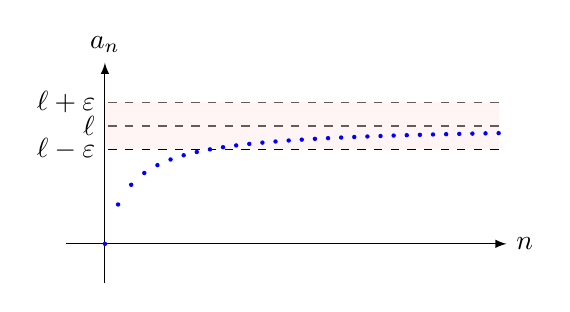
\begin{tikzpicture}
        \draw[-latex]   (-.5,0) -- (5.1,0) node[right] {$n$};
        \draw[-latex]   (0,-.5) -- (0,2.3) node[above] {$a_n$};
        \draw[thin,dashed] (5,1.8)--(0,1.8) node[left] () {$\ell+\varepsilon$};
        \draw[thick,dashed] (5,1.5)--(0,1.5) node[left] () {$\ell$};
        \draw[thin,dashed] (5,1.2)--(0,1.2) node[left] () {$\ell-\varepsilon$};
        \fill[red!10, opacity=0.4] (0,1.2) rectangle (5,1.8);
        \foreach \x in {0,...,30}
        \fill[blue] ({\x/6},{(2*\x+1)/(\x+2)-0.5}) circle(0.8pt); 
\end{tikzpicture}
\end{center}

\subsection{Rechenregeln für Grenzwerte}
Seien \(a, b\) zwei konvergente Folgen und \(c\) eine Konstante, so gelten folgende Rechenregeln:
\begin{align*}
    \lim_{n \to \infty} (c \cdot a_n) &= c \cdot \lim_{n \to \infty} a_n\\
    \lim\limits_{n \to \infty} (a_n \pm b_n) &= \lim\limits_{n \to \infty} a_n \pm \lim\limits_{n \to \infty} b_n\\
    \lim\limits_{n \to \infty} (a_n \cdot b_n) &= \lim\limits_{n \to \infty} a_n \cdot \lim\limits_{n \to \infty} b_n\\
    \lim\limits_{n \to \infty} \left(\frac{a_n}{b_n}\right) &= \frac{\lim\limits_{n \to \infty} a_n}{\lim\limits_{n \to \infty} b_n}, \quad \text{ falls } b \neq 0\\
\end{align*}

\subsection{Grenzwerte von Polynomen}
Sei \(p(n) = a_k n^k + a_{k-1} n^{k-1} + \ldots + a_1 n + a_0\) ein Polynom vom Grad \(k\) mit \(a_k \neq 0\). Dann gilt:
\[
\lim_{n \to \infty} p(n) = \begin{cases}
+\infty, & \text{falls } a_k > 0\\
-\infty, & \text{falls } a_k < 0
\end{cases}
\]

Sei \(p(n)\) und \(q(n)\) zwei Polynome vom Grad \(g_p\) bzw. \(g_q\) mit führenden Koeffizienten \(a_k\) bzw. \(b_m\). Dann gilt:
\[
\lim_{n \to \infty} \frac{p(n)}{q(n)} = \begin{cases}
0, & \text{falls } g_p < g_q\\
\frac{a_k}{b_m}, & \text{falls } g_p = g_q\\
+\infty, & \text{falls } g_p > g_q \text{ und } \frac{a_k}{b_m} > 0\\
-\infty, & \text{falls } g_p > g_q \text{ und } \frac{a_k}{b_m} < 0
\end{cases}
\]

\subsection{Wichtige Grenzwerte}
\begin{align*}
    \lim_{n \to \infty} \left(1 + \frac{1}{n}\right)^n &= e\\
    \lim_{n \to \infty} \sqrt[n]{a} &= 1, \quad a > 0\\
    \lim_{n \to \infty} q^n &= \begin{cases}
    0, & |q| < 1\\
    1, & q = 1\\
    +\infty, & q > 1\\
    \text{existiert nicht}, & q \le -1
    \end{cases}
\end{align*}

\subsection{Sandwich-Prinzip}
Seien \((a_n)\), \((b_n)\) und \((c_n)\) drei Folgen, so dass \(a_n \leq b_n \leq c_n\) für alle \(n\) ab einem gewissen Index \(n_0\). Falls \(\lim_{n \to \infty} a_n = \lim_{n \to \infty} c_n = L\) gilt, so konvergiert auch \((b_n)\) und es gilt \(\lim_{n \to \infty} b_n = L\).
